\begin{frame}
  \frametitle{Methodology}
\begin{columns}
	\begin{column}{.55\textwidth}
		\begin{block}{How does PyRe work?} 
			PyRe does the following with an input stream and facility configuration parameters: 
			\begin{itemize}
				\item Pass fuel to voloxidation.
				\item Generate efficiencies from parameters.
				\item Multiply stream by efficiency matrix.
				\item Record stream compositions.
				\item Repeat for each process.
			\end{itemize}
		\end{block}
	\end{column}
	\begin{column}{.45\textwidth}
		\begin{figure}
			\centering
			
\includegraphics[width=0.9\linewidth]{cyclus}
			\label{fig:cyclus}
		\end{figure}
	\end{column}
\end{columns} 
\end{frame}

\begin{frame}
	\frametitle{Cyclus}
    \begin{block}{What is Cyclus?}
    	Cyclus is a modular agent based fuel cycle simulator for tracking commodity transactions
    	between facilities.
    \end{block}
	\begin{figure}
		\centering
		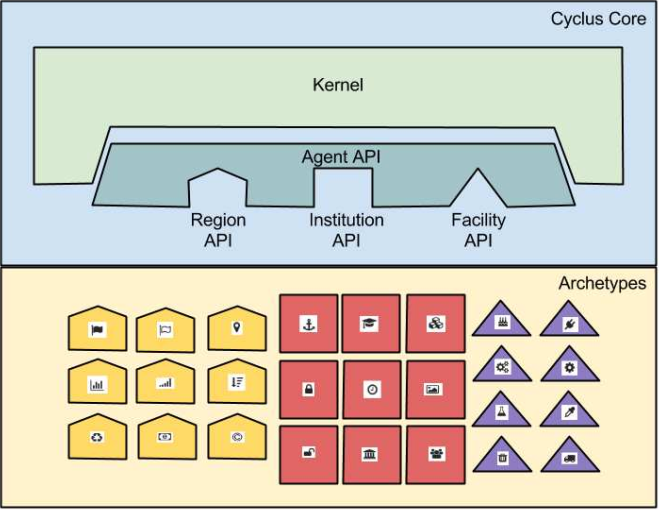
\includegraphics[width=0.6\linewidth]{Cyclus_graph}
		\caption{Cyclus Archetype framework and API\ref{cyclus-dev}.}
	\end{figure}
\end{frame}

\begin{frame}
\frametitle{Why Cyclus?}
	Cyclus allows the construction of specific scenarios through the addition of archetypes. These archetypes are
	modular and the transactions can be tracked.
	\begin{figure}
		\centering
		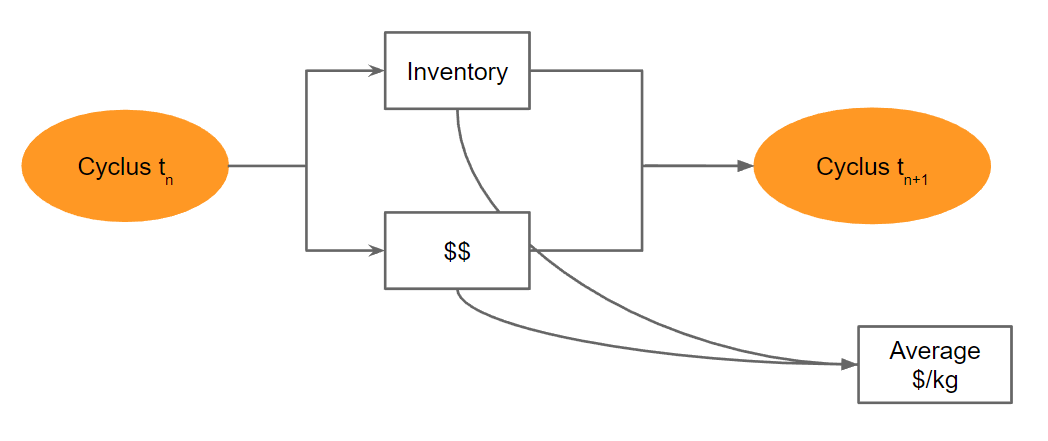
\includegraphics[width=0.9\linewidth]{cyclus-material-track}
		\caption{Cyclus tracks material flow through the fuel cycle.}
		\label{fig:tracking}
	\end{figure}
\end{frame}

\begin{frame}
\frametitle{Assumptions}
\begin{columns}
	\begin{column}{.45\textwidth}
		\begin{block}{Cyclus Requirements} 
			\begin{itemize}
				\item Modular.
				\item Time step $\geq$ 1 month
				\item Streams must be in a
				trade-able form.
				\item Parameters are constant for the simulation.
				\begin{itemize}
					\item Equation input toolkit under development.
				\end{itemize}
				\item Diversion detection must be added after.
			\end{itemize}
		\end{block}
	\end{column}
	\begin{column}{.55\textwidth}
		\begin{figure}
			\centering
			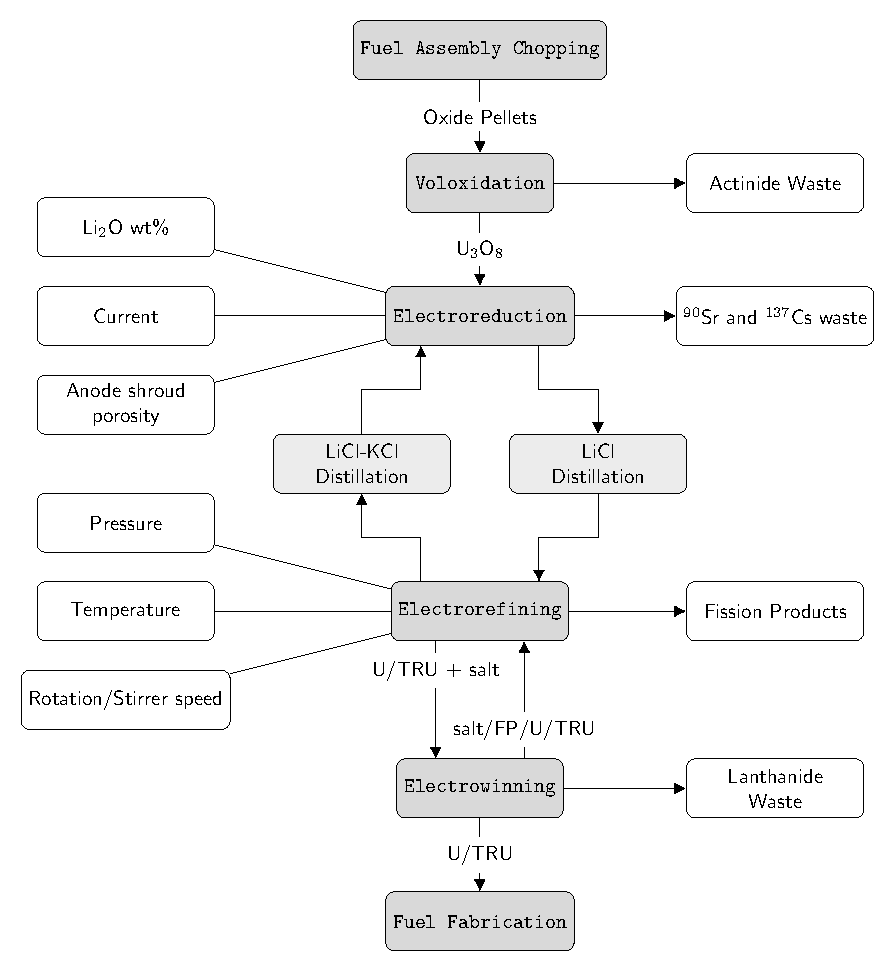
\includegraphics[width=0.9\linewidth]{flowchart}
			\caption{PyRe material flowchart \ref{borelli}.}
			\label{fig:cyclus}
		\end{figure}
	\end{column}
\end{columns} 
\end{frame}

\begin{frame}
\frametitle{Subprocesses}
\begin{columns}
	\begin{column}{.5\textwidth}
		\begin{figure} 
			\centering
			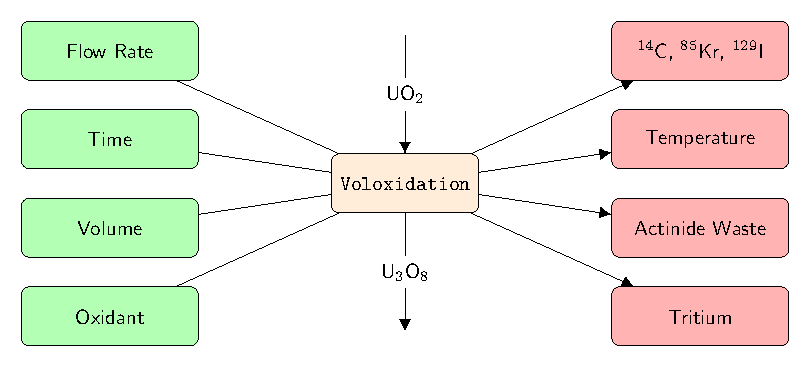
\includegraphics[width=0.9\linewidth]{volox}
			\caption{Voloxidation material balance area \ref{jupin}.}
			\label{fig:volox}
		\end{figure}
		\begin{figure} 
			\centering
			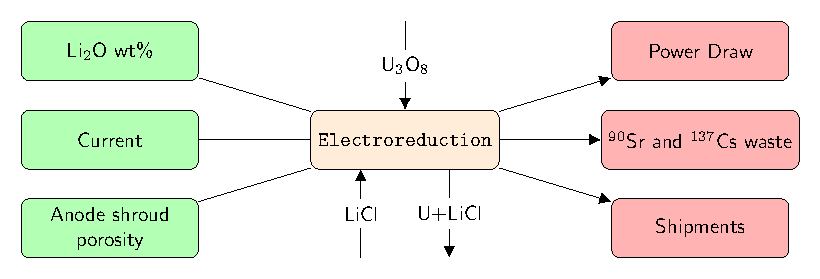
\includegraphics[width=0.9\linewidth]{reduction}
			\caption{Reduction material balance area \ref{kaeri}.}
			\label{fig:reduction}
		\end{figure}
	\end{column}
	\begin{column}{.5\textwidth}
		\begin{figure}
			\centering
			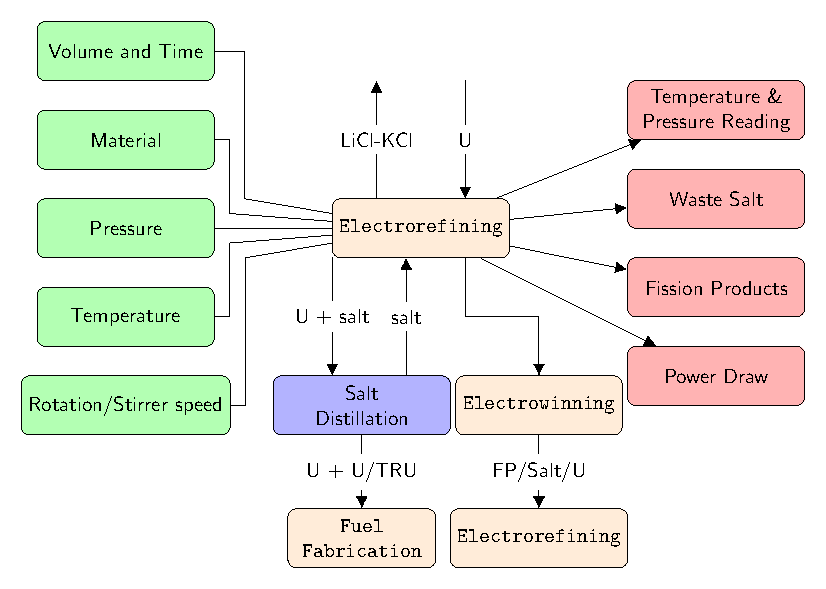
\includegraphics[width=0.9\linewidth]{refining}
			\caption{Refining material balance area \ref{kaeri}.}
			\label{fig:refining}
		\end{figure}
		\begin{figure} 
			\centering
			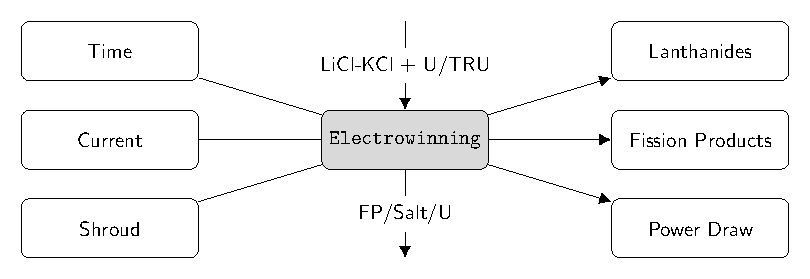
\includegraphics[width=0.8\linewidth]{winning}
			\caption{Winning material balance area.}
			\label{fig:winning}
		\end{figure}
	\end{column}
\end{columns} 
\end{frame}